	
% .:: Laden der LaTeX4EI Formelsammlungsvorlage
\documentclass[fs, footer]{latex4ei}

% Dokumentbeginn
% ======================================================================
\begin{document}


% Aufteilung in Spalten
\begin{multicols*}{4}
\fstitle{Power Electronic Systems I}


\section{Useful knowledge}

\sectionbox{
\subsection{Sinus, Cosinus \quad $\sin^2(x) \bs + \cos^2(x) = 1$}
\setlength{\tabcolsep}{4pt}
\tablebox{
\begin{tabular*}{\columnwidth}{@{\extracolsep\fill}c|c|c|c|c||c|c|c|c@{}} \ctrule
$x$ & $0$ & $\pi / 6$ & $\pi / 4$ & $\pi / 3$ & $\frac{1}{2}\pi$ & $\pi$ & $1\frac{1}{2}\pi$ & $2 \pi$ \\
$\scriptstyle{ \varphi }$ & $\scriptstyle{0^\circ}$ & $\scriptstyle{30^\circ}$ & $\scriptstyle{45^\circ}$ & $\scriptstyle{60^\circ}$ & $\scriptstyle{90^\circ}$ & $\scriptstyle{180^\circ}$ & $\scriptstyle{270^\circ}$ & $\scriptstyle{360^\circ}$ \\ \cmrule
$\sin$ & $0$ & $\frac{1}{2}$ & $\frac{1}{\sqrt{2}}$ & $\frac{\sqrt 3}{2}$ & $1$ & $0$ & $-1$ & $0$ \\
$\cos$ & $1$ & $\frac{\sqrt 3}{2}$ & $\frac{1}{\sqrt 2}$ & $\frac{1}{2}$ & $0$ & $-1$ & $0$ & $1$ \\     
$\tan$ & $0$ & $\frac{\sqrt{3}}{3}$ &	$1$	&	$\sqrt{3}$ & $\pm \infty$ & $0$ & $\mp \infty$ & $0$\\ \cbrule
\end{tabular*} }\\
\begin{tabular*}{\columnwidth}{@{\extracolsep\fill}ll@{}}
	Additionstheoreme &  Stammfunktionen\\
 	$\cos (x - \frac{\pi}{2}) = \sin x$ & $\int x \cos(x) \diff x = \cos(x) + x \sin(x)$\\
 	$\sin (x + \frac{\pi}{2}) = \cos x$ & $\int x \sin(x) \diff x = \sin(x) - x \cos(x)$\\
 	$\sin 2x = 2 \sin x \cos x $  & $\int \sin^2(x) \diff x = \frac12 \bigl(x - \sin(x)\cos(x) \bigr)$\\ 
 	$\cos 2x = 2\cos^2 x - 1$  & $\int \cos^2(x) \diff x = \frac12 \bigl(x + \sin(x)\cos(x) \bigr)$\\
 	$\sin(x) = \tan(x)\cos(x)$ & $\int \cos(x)\sin(x) = -\frac12 \cos^2(x)$ \\
\end{tabular*}\\
}

\sectionbox{
	\subsection{Integrals $\int e^x\;\mathrm{d} x = e^x = (e^x)'$}
	partial integration: $\int uw'=uw-\int u'w$\\
	substitution: $\int f(g(x)) g'(x)\,\mathrm dx=\int f(t)\, \mathrm dt$\\
	\tablebox{
	\renewcommand{\arraystretch}{1.6} 
	\begin{tabular*}{\columnwidth}{@{\hspace{5mm}}c@{\extracolsep\fill}c@{\extracolsep\fill}c@{\hspace{5mm}}} \ctrule
		$F(x)$ & $f(x)$ & $f'(x)$ \\ \cmrule
		$\frac{1}{q+1}x^{q+1}$ & $x^q$ & $qx^{q-1}$ \\
		\raisebox{-0.2em}{$\frac{2\sqrt{ax^3}}{3}$} & $\sqrt{ax}$ & \raisebox{0.2em}{$\frac{a}{2\sqrt{ax}}$}\\
		$x\ln(ax) -x$ & $\ln(ax)$ & $\textstyle \frac{a}{x}$\\
		%e^x & e^x & e^x \\
		$\frac{1}{a^2} e^{ax}(ax- 1)$ & $x \cdot e^{ax}$ & $e^{ax}(ax+1)$ \\
		$\frac{a^x}{\ln(a)}$ & $a^x$ & $a^x \ln(a)$ \\
		$-\cos(x)$ & $\sin(x)$ & $\cos(x)$\\
		$\cosh(x)$ & $\sinh(x)$ & $\cosh(x)$\\
		$-\ln |\cos(x)|$ & $\tan(x)$ & $\frac{1}{\cos^2(x)}$ \\ \cbrule
	\end{tabular*} }\\
	
	$\int e^{at} \sin(bt) \diff t = e^{at} \frac{a \sin(bt) + b \cos(bt)}{a^2 + b^2}$\\
	\begin{tabular*}{\columnwidth}{@{\extracolsep\fill}ll@{}}
	$\int \frac{\diff t}{\sqrt{at+b}} = \frac{2 \sqrt{at+b}}{a}$ & $\int t^2 e^{at} \diff t = \frac{(ax-1)^2+1}{a^3} e^{at}$\\
	$\int t e^{at} \diff t = \frac{at-1}{a^2} e^{at}$ & $\int x e^{ax^2} \diff x = \frac{1}{2a} e^{ax^2}$\\
	\end{tabular*}
}
\sectionbox{
	\subsection{Fourier decomposition}
	
	is the decomposition of a function $f\in C(T)$ in a series of $\sin$ and $\cos$ fuctions.\\
	$C(T):$ $T$-periodic, stetig fortsetzbar\\
	$f$ ist $T$-periodic, if $f(x+T) = f(x)$ $\ra$ also $n \cdot T$ periodic.
	
	\subsubsection{Decompositon in fourier series $f(x) \sim F(x)$}


	 Calculation of the fourier cooeficients for  $f \in C(T)$:\\
	$a_k,b_k \in \R$: \quad $ \Big\{ { ^{\textstyle a_k}_{\textstyle b_k}} = \frac{2}{T} \int\limits_{-\frac{T}{2}}^{\frac{T}{2}} f(x) \Big\{ {}^{\textstyle \cos} _{\textstyle \sin} \left(k \frac{2\pi}{T} x \right) \diff x$\\
	
	
	Calculation of the Fourier series $F$ for $f$:  \\
	$ F(x) = \frac{a_0}{2} + \sum\limits_{k=1}^\infty a_k \cos \left(k \frac{2\pi}{T} x \right) + b_k \sin \left( k \frac{2\pi}{T} x \right) $\\
	

	For symmetric functions:	
	\begin{itemize}
	\item $f \in C(T)$ even (achsensym.) function: $c_k = c_{-k}$ \\
	$b_k = 0$ und $a_k = \frac{4}{T} \int_{0}^{T/2} f(x) \cos \left(k \frac{2\pi}{T} x \right) \diff x$
	\item $f \in C(T)$ uneven (punktsym.) function: $c_k = -c_{-k}$\\
	$a_k = 0$ und $ b_k = \frac{4}{T} \int_{0}^{T/2} f(x) \sin \left(k \frac{2\pi}{T} x \right) \diff x$
	\end{itemize}
}


\sectionbox{	
\subsection{LaPlace transformation \quad $\mathcal L\bigl(f(t)\bigr) = F(s)$}
% ==============================================================================================================	
	$f(t) \LT F(s) := \int\limits_0^\infty f(t) \exp(-st) \diff t$\\
	\\
	\everymath{\displaystyle}	% Formeln ab hier groß Schreiben
	\begin{tabular}{rl|rl}
		$1$ & $\LT \frac{1}{s}$ & $\delta(t-t_0)$ &$\LT e^{-s t_0}$\\[0.2em]
		$t^n$ &$\LT \frac{n!}{s^{n+1}}$ & $e^{at}$  &$\overset{s > a}{ \LT } \frac{1}{s-a}$\\[0.5em] 
		$\sin(t)$ &$\LT \frac{1}{s^2 + 1}$ & $\cos(t)$ &$\LT \frac{s}{s^2 + 1}$\\[0.5em]
		$\sin(\omega t)$ &$\LT \frac{\omega}{s^2 + \omega^2}$ & $\cos(\omega t)$ &$\LT \frac{s}{s^2 + \omega^2}$\\[0.5em]
		\multicolumn{4}{l}{ $e^{-at} \sin(\omega t) \LT \frac{\omega}{(s+a)^2+\omega^2}$} \\
		\multicolumn{4}{l}{ $e^{-at} \cos(\omega t) \LT \frac{s+a}{(s+a)^2+\omega^2}$}\\ 		

	\end{tabular}\\
	\everymath{\textstyle}
	Liniarity: $\alpha f(t) + \beta g(t) \LT \alpha F(s) + \beta G(s)$\\
	Similarity: $f(ct) \LT \frac{1}{c} F\bigl(  \frac{s}{c} \bigr)$\\
	Derivative in time domain:\\
	$f'(t) \LT s F(s) - f(0)$ \\
	 $f''(t) \LT s^2 F(s) - sf(0) - f'(0)$\\
	$f^{(n)} \LT s^n F(s) - s^{n-1} f(0) - s^{n-2} f'(0) \ldots - f^{(n-1)}(0)$\\
	Integral in time domain: $\int_0^t f(x) \diff x \LT \frac{1}{s} F(s)$\\
	Derivative in LP domain: $(-t)^n f(t) \LT F^{(n)} (s)$\\
	Time shift: $f(t-a)\heavi(t-a) \LT e^{-as} F(s)$\\

	Damping: $e^{-at} f(t) \LT F(s+a)$\\
	Convolution: $(f * g)(t) := \int_0^t f( t - \tau) g(\tau) \diff \tau$ $\LT F(s) \cdot G(s)$\\
	Inverse: $f(t) = \frac{1}{2\pi \i} \int\limits_{\gamma - \i \infty}^{-\gamma + \i \infty} F(s) \exp(st) \diff s$\\
	



}
\section{Power Semiconductor Switches}
\sectionbox{
\subsection{Diodes}
Types:  Schottky, Fast-recovery, Line-frequency

States:
\begin{itemize}
	\item forward bias: forward voltage $\approx 1 \si{\volt}$
	\item reverse biased: small leakage current, until reverse-bias voltage is reached
\end{itemize}

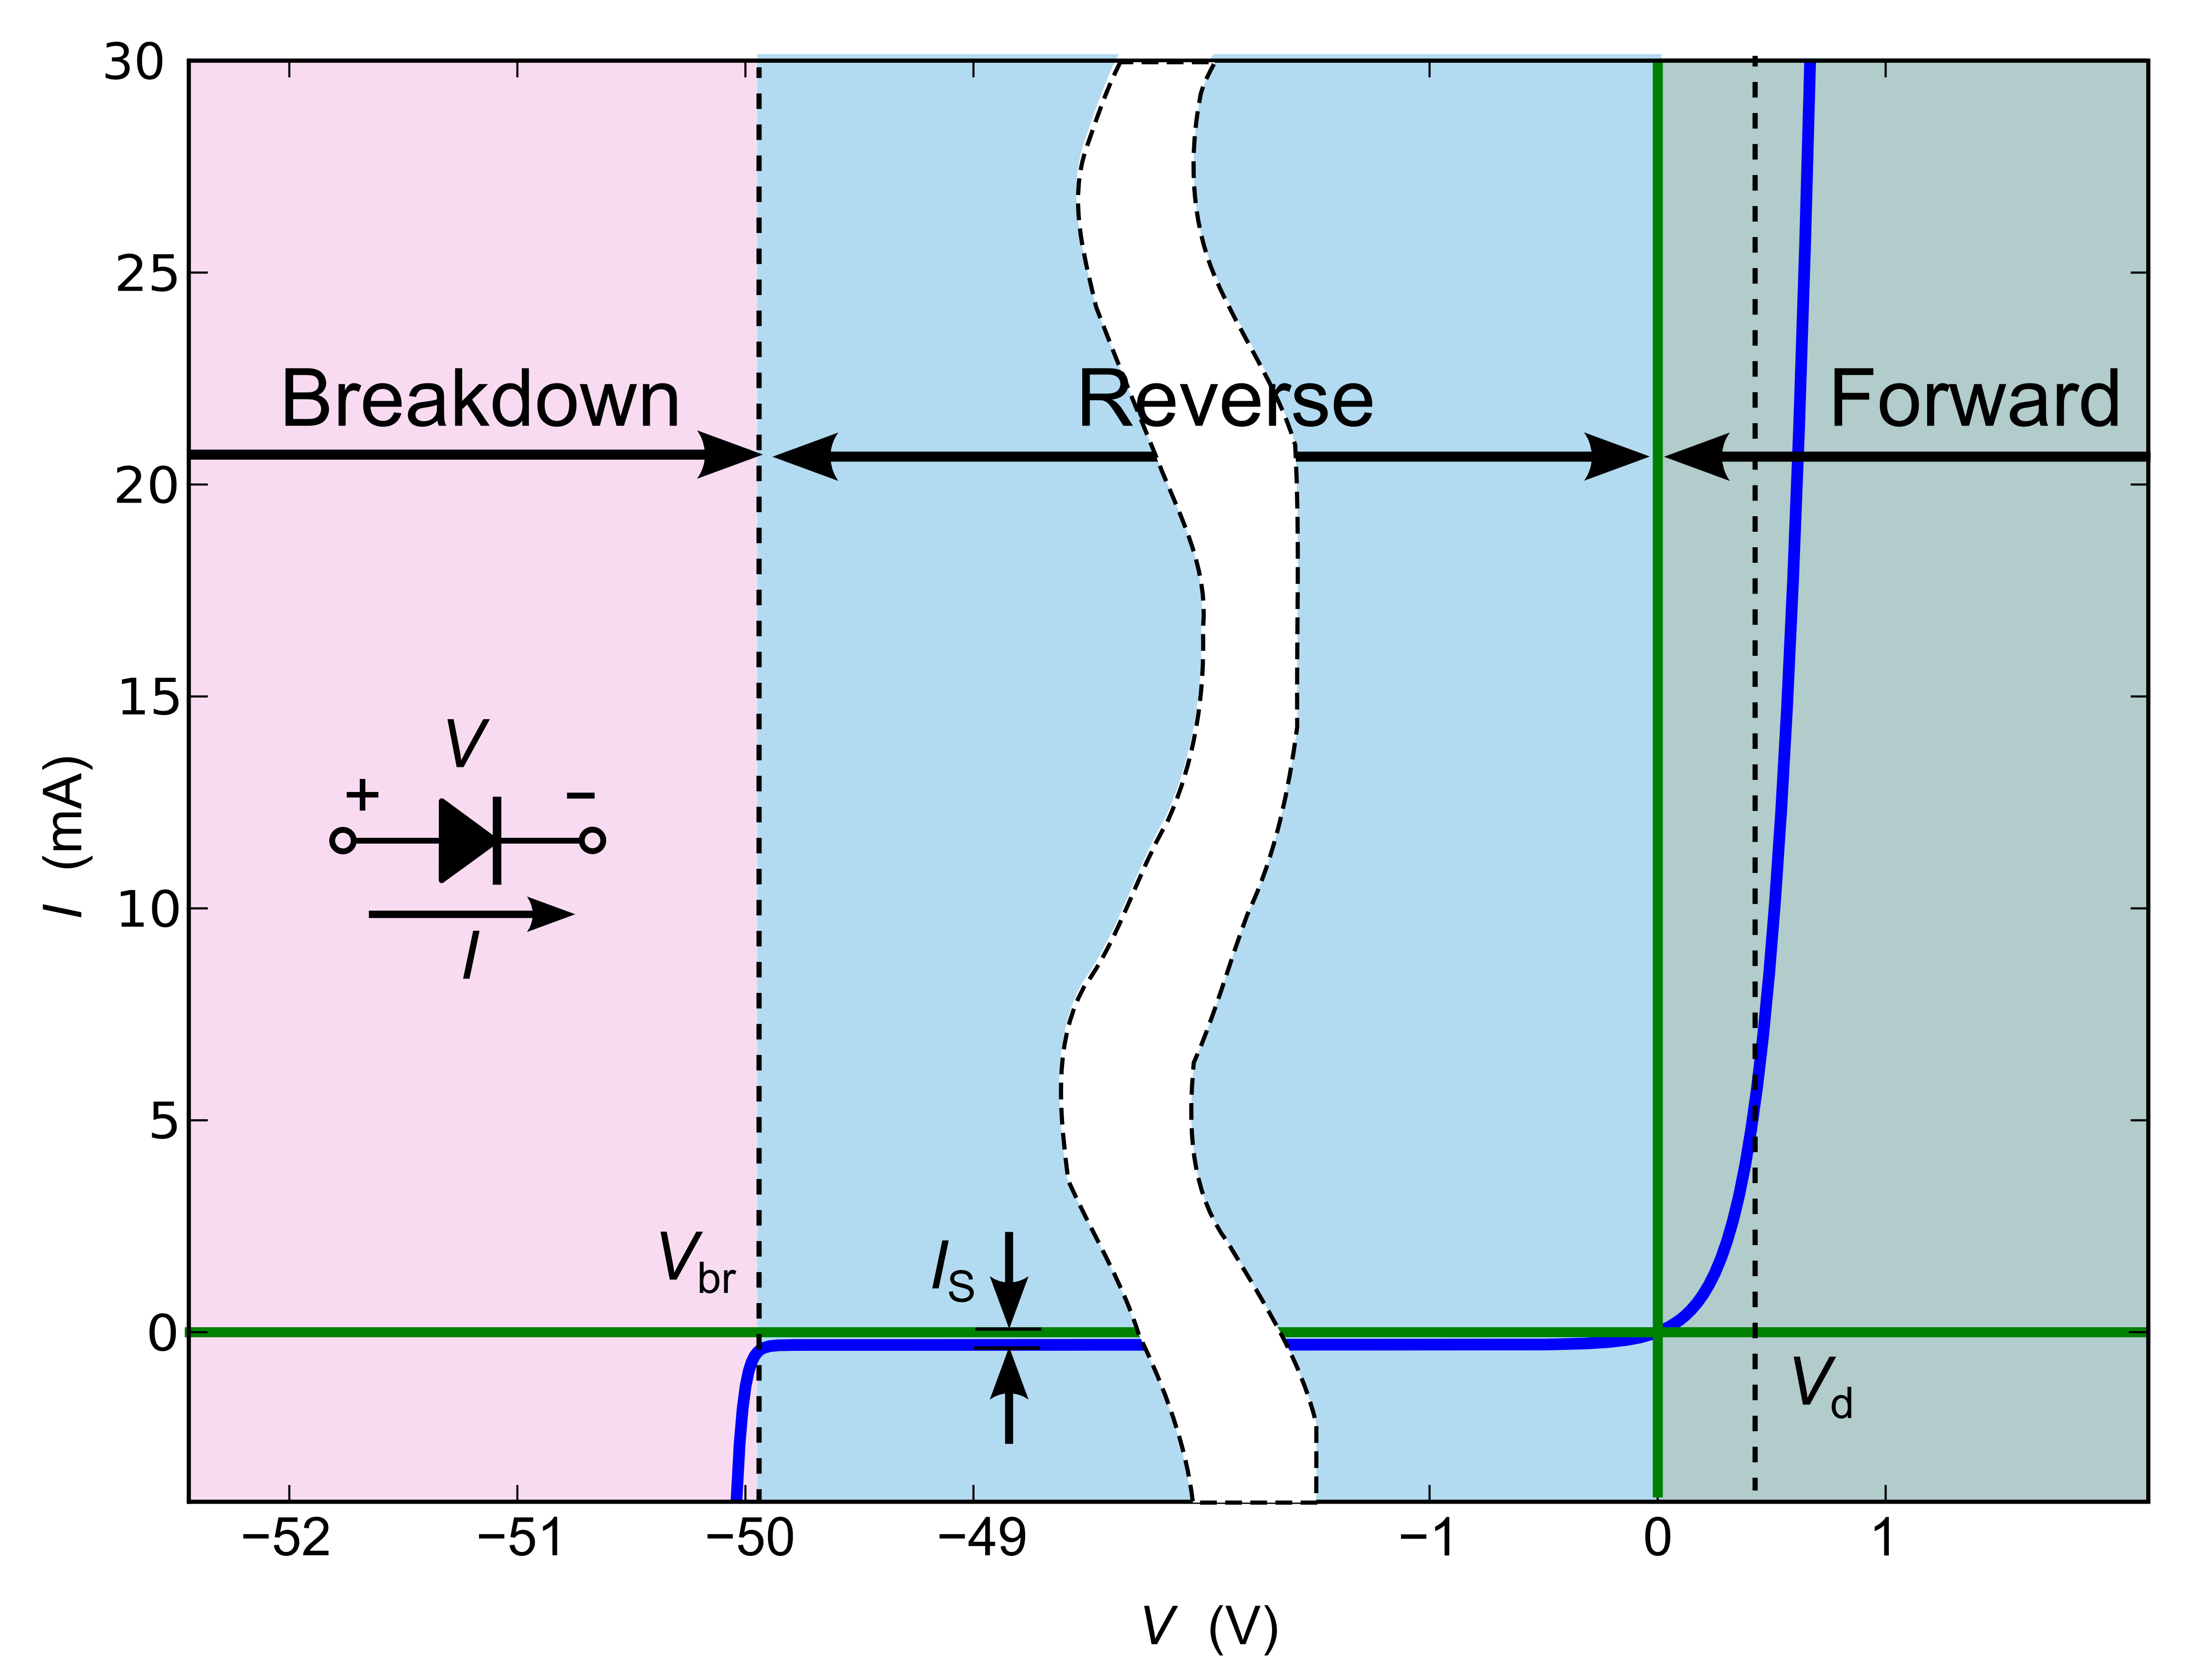
\includegraphics[width=\columnwidth]{./img/Diode_current_wiki.png}

\symbolbox{
	\begin{tabular*}{\columnwidth}{@{\extracolsep}ll@{}}
		$t_{\ir rr}$ & reverse recovery time \\
	\end{tabular*}
}
}
\sectionbox{
\subsection{Thyristors}  

States:
\begin{itemize}
	\item reverse biased: small leakage current, until reverse-bias voltage is reached
	\item forward biased - off: blocks forward polarity
	\item forward biased - on: pulse of positive gate current $\Ra$ forward voltage drops to $\approx 1-3 \si{\volt}$
\end{itemize}
Thyristor cannot be turned off by the gate!

\symbolbox{
	\begin{tabular*}{\columnwidth}{@{\extracolsep}ll@{}}
		$t_{\ir q}$ & turn-off time interval: between zero-crossing of $i$ and $u$\\
	\end{tabular*}
}

Characteristics:
\begin{itemize}
	\item voltage ratings
	\item turn-off time $t_{\ir q}$
	\item forward voltage drop
	\item rise of current at turn-on $\diff i / \diff t$
	\item rise of voltage at turn-off $\diff v / \diff t$
\end{itemize}

Types:
\begin{itemize}
	\item Phase-control thyristors
	\item Inverter-grade thyristors
	\item Light-activated thyristors
\end{itemize}
}
\subsection{Controllable Switches} 
% Ende der Spalten
\end{multicols*}

% Dokumentende
% ======================================================================
\end{document}

% ToDos:

